% !TEX program = latexmk
% !TEX options = -cd -r "%DIR%/auxiliary/latexmkrc" -synctex=1 -interaction=nonstopmode -halt-on-error "%DOC%"
\makeatletter
\def\input@path{{auxiliary/}}
\makeatother
\documentclass[conference]{IEEEtran}
\IEEEoverridecommandlockouts
% The preceding line is only needed to identify funding in the first footnote. If that is unneeded, please comment it out.
%Template version as of 6/27/2024

\usepackage{cite}
\usepackage{amsmath,amssymb,amsfonts}
\usepackage{algorithmic}
\usepackage{graphicx}
\graphicspath{{images/}{auxiliary/}}
\usepackage{textcomp}
\usepackage{xcolor}
\usepackage{url}

\usepackage{tikz}
\usepackage{xcolor}

\def\BibTeX{{\rm B\kern-.05em{\sc i\kern-.025em b}\kern-.08em
    T\kern-.1667em\lower.7ex\hbox{E}\kern-.125emX}}
\begin{document}

\title{Conference Paper Title*\\
{\footnotesize \textsuperscript{*}Note: Sub-titles are not captured for https://ieeexplore.ieee.org  and
should not be used}
\thanks{Identify applicable funding agency here. If none, delete this.}
}

\author{\IEEEauthorblockN{Jaime Mosquera}
\IEEEauthorblockA{\textit{Student} \\
\textit{University of Minho}\\
Braga, Portugal \\
pgxxxxx@uminho.pt}
\and
\IEEEauthorblockN{Jorge Marco}
\IEEEauthorblockA{\textit{Student} \\
\textit{University of Minho}\\
Braga, Portugal \\
pg65303@uminho.pt}
}

\maketitle

\section{Introduction}
In this work our goal is to anayze and optimise a caculation of classical molecular dynamics (MD). It is
based in an original code from~\cite{foleylab-md}.

% Background for the supplied MD.cpp; implementation observations are kept explicit.
\section{Background}
\label{sec:background}

Classical molecular dynamics follows the motion of $N$
interacting particles by numerically integrating Newton's
equations of motion. Only the expressions needed for the
parallelization study are summarized here.

Two particles separated by a distance $r>0$ interact through the
Lennard-Jones (LJ) potential~\cite{jones1924}
\begin{equation}
 V(r)=4\varepsilon
 \left[
 \left(\frac{\sigma}{r}\right)^{12}
 -
 \left(\frac{\sigma}{r}\right)^6
 \right],
 \label{eq:lj-potential}
\end{equation}
where $\varepsilon$ and $\sigma$ set the energy and length scales
(Fig.~\ref{fig:lj-potential}).

\begin{figure}[htbp]
\centering
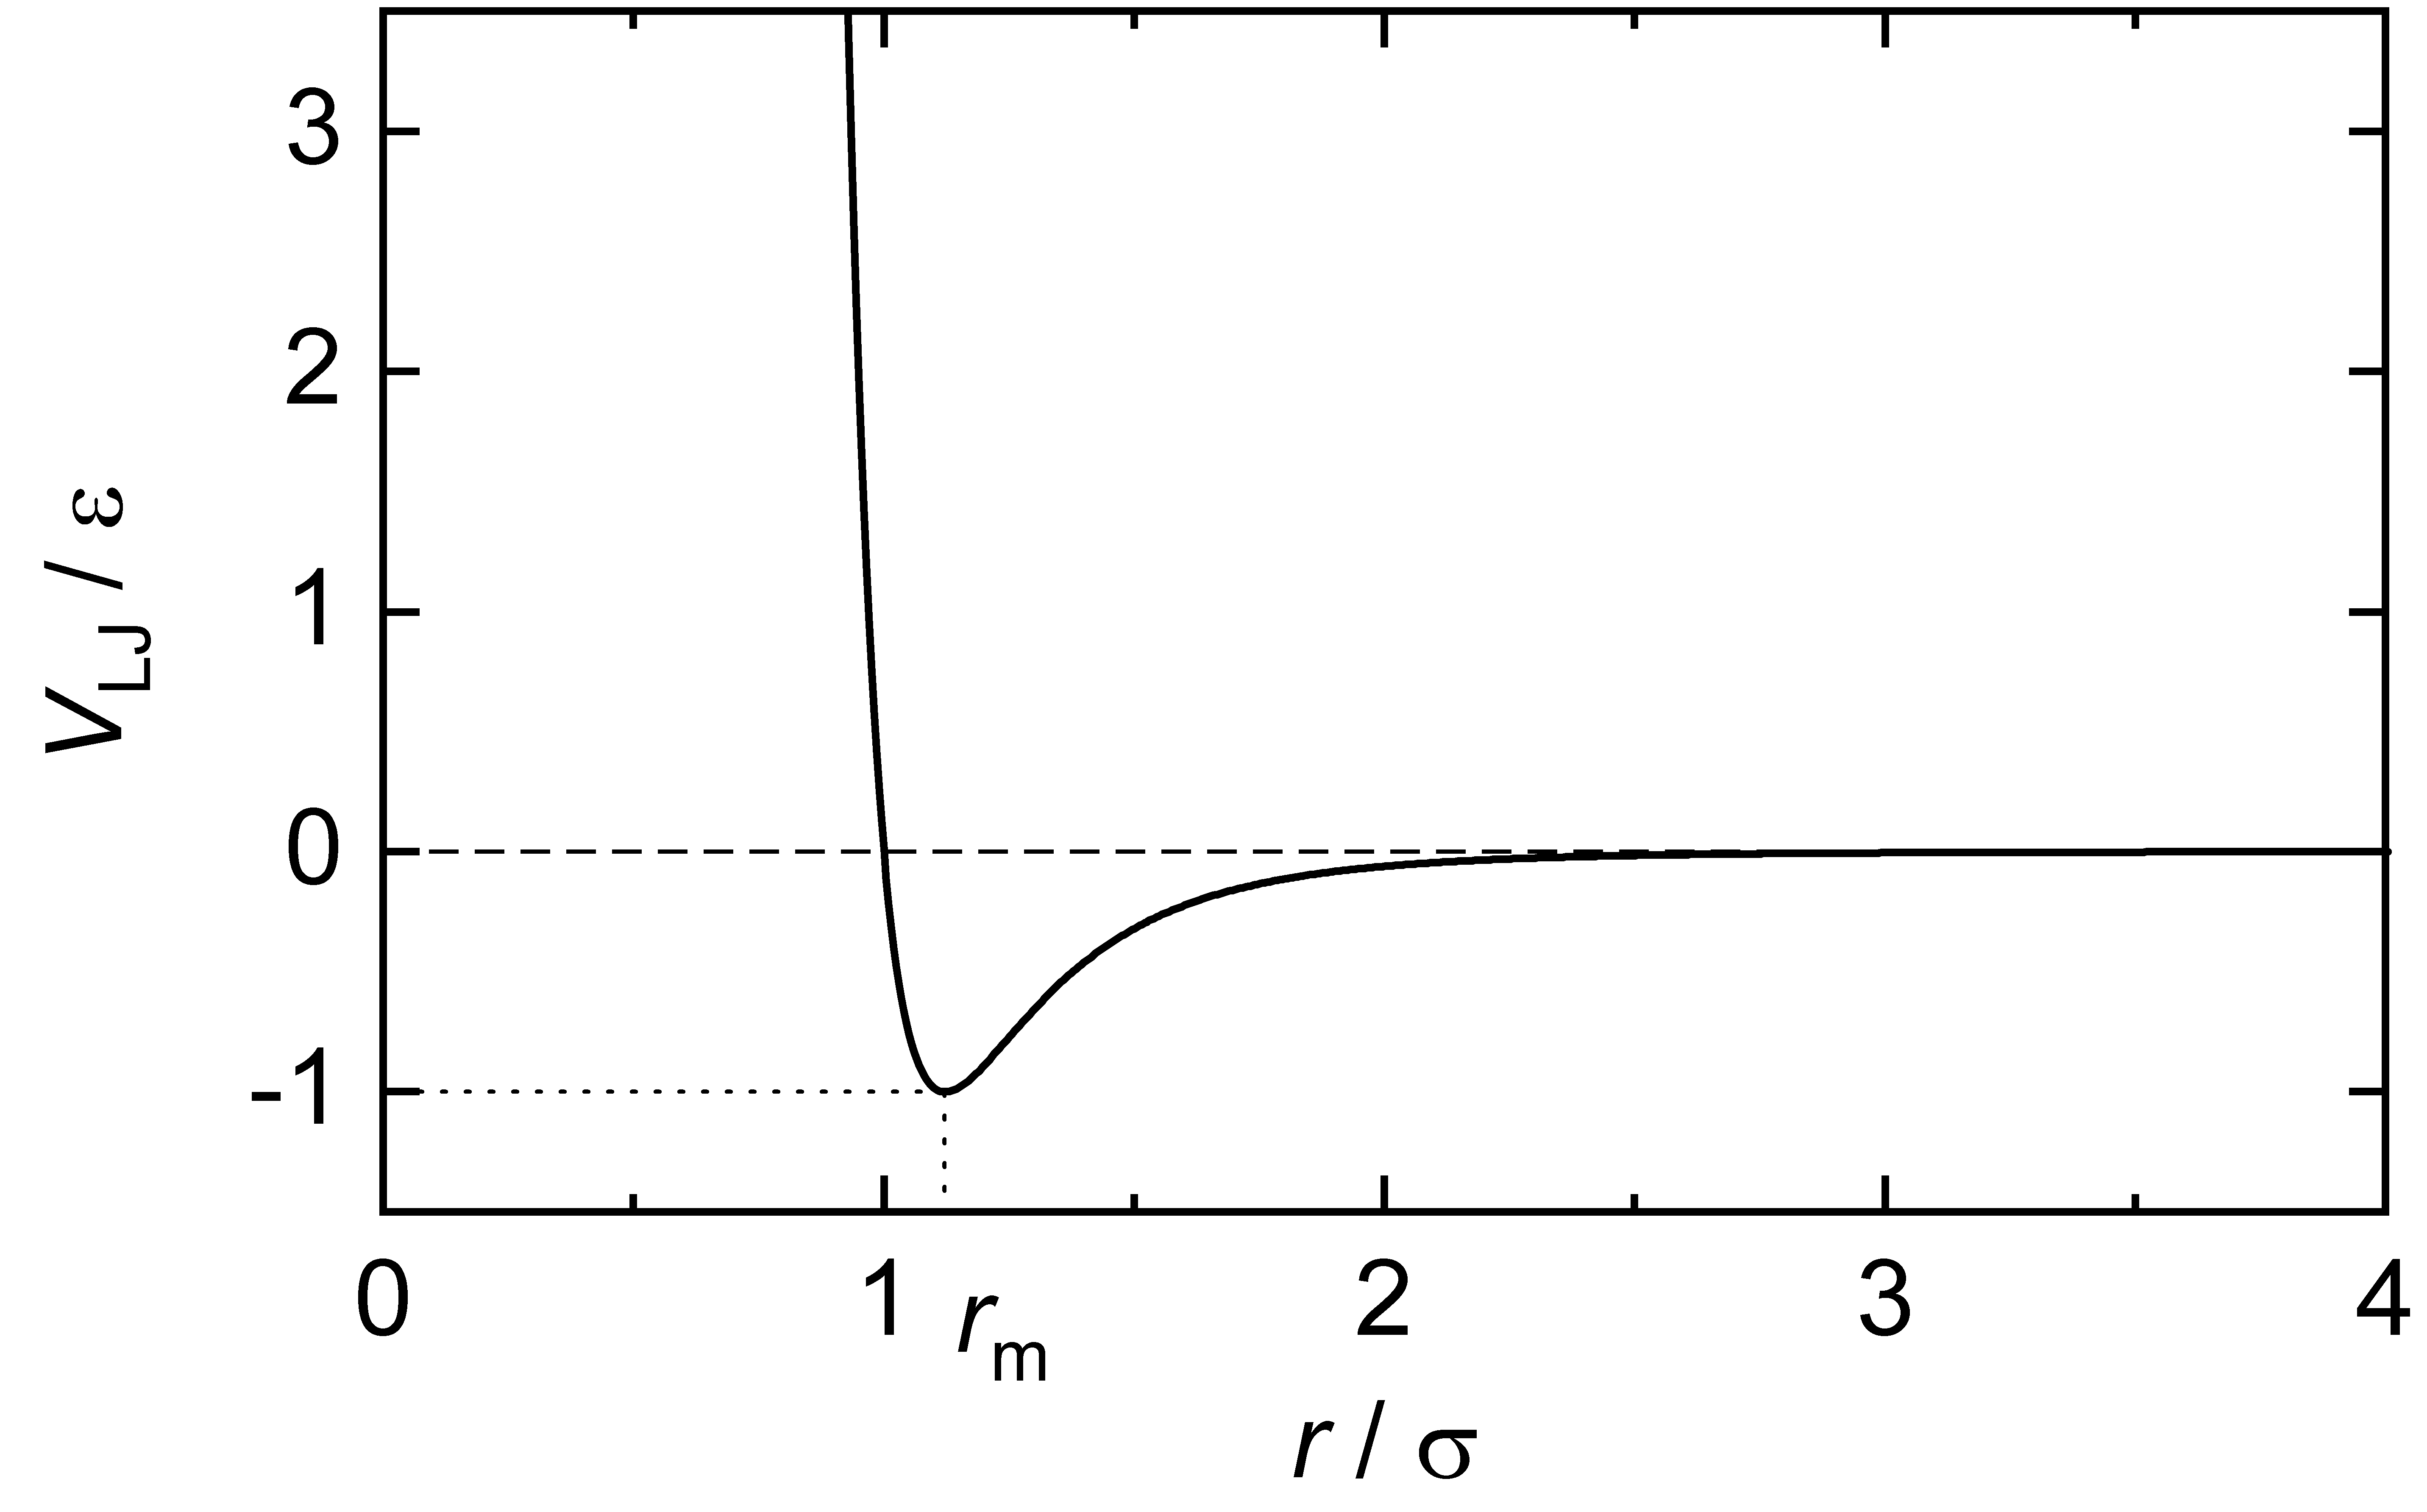
\includegraphics[width=\columnwidth]{lennard-jones-potential.png}
\caption{Lennard-Jones potential $V(r)$ as a function of the
interparticle distance~\cite{lj-figure}. Image by TimeStep89,
licensed under CC BY 4.0
(\protect\url{https://creativecommons.org/licenses/by/4.0/}); unmodified.}
\label{fig:lj-potential}
\end{figure}

Since interactions are pairwise and symmetric, the number of
unique interactions is
\begin{equation}
 |\mathcal S|=\frac{N(N-1)}{2}.
 \label{eq:lj-pair-count}
\end{equation}

In reduced LJ units, the acceleration contribution to particle
$i$ from particle $j$, with $\mathbf r_{ij}=\mathbf r_i-\mathbf r_j$
and $r_{ij}=\|\mathbf r_{ij}\|$, is
\begin{equation}
 \boxed{
 \mathbf g_{ij}
 =
 24\left(
 \frac{2}{r_{ij}^{14}}
 -
 \frac{1}{r_{ij}^{8}}
 \right)\mathbf r_{ij},
 }
 \label{eq:lj-reduced-acceleration}
\end{equation}
and the total acceleration of particle $i$ is
$\mathbf a_i=\sum_{j\neq i}\mathbf g_{ij}$.

\section{Methodology}
\label{sec:methodology}

The optimization follows five steps. 
\subsection{Identify code blocks with high computation time.}The first step profiles
the original code to identify the code blocks that consume most
of the execution time. Optimizing the slowest blocks is the optimal
optimizing strategy according to Amdahl's law~\cite{amdahl1967}.
\begin{equation}
 S=\frac{1}{(1-p)+p/s}\le\frac{1}{1-p}.
 \label{eq:amdahl}
\end{equation}
According to this law, optimising the blocks with the largest $p$ yields
the highest attainable speedup

\section{Results}
Profiling of the original code identifies the functions \texttt{Potential()} and
\texttt{computeAccelerations()} as the most expensive, consuming 56\% and 41\% of
the total execution time, respectively.

\bibliographystyle{ieeetr}
\bibliography{references}

\end{document}
